\documentclass{article}
\usepackage{hyperref}
\usepackage[a4paper, margin=2.5cm]{geometry}
\usepackage{graphicx}
\begin{document}
\title{Task 5: Jarnik-Prim on Sample-MST with Filter}
\author{Lucas Alber (***REMOVED***), Noah Wahl (***REMOVED***)}
\maketitle

\section{Implementation}

Every step of our implementation was carefully evaluated using micro benchmarks.
The time measurement code can be found in our git history, we removed it for our final benchmarks.
The following subsections present our findings.

\subsection{Sampling}
\textbf{Problem:} We receive undirected edges as directed edges in both directions from the graph generator.
However, the sampling would be far easier if these edges were only present in one direction, to prevent accidentally sampling duplicates.

\noindent \\
\textbf{Solution:} We went through multiple sampling strategies:

\begin{enumerate}
\item \texttt{std::mt19937}: Select an edge \texttt{e if e.tail < e.head} with probability $p = n / \sqrt{n \times m} = \sqrt{n / m}$.
This turned out to be very slow because branch miss-predictions on these conditions are very common and we have to iterate over the whole edge list.

\item \texttt{std::mt19937}: Select $\sqrt{n \times m}$ edges \texttt{edge\_list[x\_i]} where \texttt{x\_i} is sampled uniformly from \texttt{[0, edge\_list.size() - 1]}.
This way we may sample edges twice, but we found this to not diminish the quality of the sample.

\item \texttt{XORShift128}: Same as 2. but with a faster random number generator.
We could not detect any compromise in quality.

\item Deterministic Sampling: Select every \texttt{edge\_list.size() / $\sqrt{n \times m}$}-th edge from the edge list.
This was more than an order of magnitude faster than relying on random number generators at no disadvantage to the quality of the sample.
So we settled for this strategy in our final implementation.
\end{enumerate}

\subsection{Graph Representation}
We use single undirected edges where possible and only add reverse edges during the adjacency array buildup for the Jarnik-Prim subroutine.
The edges in the adjacency array are reduced to weight-head pairs instead of carrying the tail as well.

\subsection{Range Maximum Queries (RMQ)}
We expand the levels to the next power of two allowing for efficient shift operations instead of multiplications.
This also eliminates special cases in the buildup. We also flattened the levels into one single array.

To speed up the filter loop condition for including edges between components, we set the weight of the root node in each component to $\inf$.
In this regard we deviate from the paper where the weight of the root node is set to zero.
This way, queries across boundaries return $\inf$ and the condition \texttt{e.weight < query(e)} evaluates to true.

\subsection{Jarnik-Prim}
Our Jarnik-Prim implementation is very straight forward. We use a specialized version for computing the minimum spanning forest for our sampled edges and combine data that is accessed together to minimize cache misses. For edge priorities we use an indexed priority queue implementation which turned out to be faster than \texttt{std::priority\_queue}, especially for dense graphs.

\subsection{Filter Loop}
The filter loop turned out to be the main bottleneck because we need to check the filter condition for each edge. However, through the aforementioned techniques we reduced the number of computations to a minimum. Additionally, we split the query on the range maximum query data structure to allow for short-circuit evaluation because in this case cache misses (on the RMQ data structure) were more expensive than branch miss-predictions.

\subsection{Exploit Simple Instances}
\label{sec:simple_instances}
Finally, our algorithm decides based on the expected runtime of Jarnik-Prim and IMaxFilter whether to run only a single Jarnik-Prim iteration or run the full IMaxFilter algorithm which can provide a speedup of two for small instances.

\subsection{Parallel IMaxFilter}
We added a simple parallel implementation of our IMaxFilter that uses OpenMP to speed up the filter loop.

\section{Testing}
To test our data structures and algorithms we added tests using the Google Test Framework.

\section{Experiments}

\subsection{Setup}
Our implementation was evaluated on a machine running Arch GNU/Linux 64bit on Linux 5.18.14 with an AMD Ryzen 5800X, 8 Cores (16 Threads) @ 3800 MHz and 4 $\times$ 8 GB DDR4 RAM @ 3400 MT/s.
We used GCC 12.1.0 to compile the code and did not change any flags.

\subsection{Evaluation}

For our evaluation we varied the number of nodes, the distribution of weights and the density of the benchmark graphs.

\noindent \\
Figure \ref{fig:13_21_1_64_2147483647_1_2_p3} shows the time per edge in relation to the number of nodes with a double-log scale.
The Jarnik-Prim-based algorithms take more time per edge with an increasing number of nodes while the implementation of Kruskal's algorithm remains nearly constant (nearly, because the Union-Find data structure depends on the number of nodes).
We observed a similar behavior for all other configurations and therefore omit these plots here.
They can be found in the \texttt{/plots} directory.

\noindent \\
Comparing Figure \ref{fig:13_16_1_2048_2147483647_1_2} and \ref{fig:13_16_1_2048_255_1_2} points out the effects of increasing the range of different weights.
Because Kruskal's algorithm sorts the edges on these weights, it experiences a noticeable slowdown when the range of weights is larger.
The Jarnik-Prim-based algorithms do not sort the edges by weights and therefore do not suffer from this.

\noindent \\
Lastly, we compared different graph densities by raising the average degree.
All figures present a similar picture.
For the numbers in this section we refer to Figure \ref{fig:13_16_1_2048_2147483647_1_2}.
The IMaxFilter algorithm was intended to be used on dense graphs and our evaluation shows that in these configurations it really does outperform the other algorithms.
Because of memory limitations we could only evaluate high density graphs with up to $2^{16}$ nodes.
Additionally, the graph generator was not able to produce high density graphs without running for a very long time.
Therefore, our maximum evaluated density is $\frac{2^{13} 2^{11}}{2^{13} (2^{13}-1)} \approx \frac{1}{4}$ for the graphs with the fewest nodes.
All Figures show a similar picture: For very small densities ($\leq 0.0005$) Kruskal performs best, but then Jarnik-Prim-based algorithms pull ahead very quickly.
Once IMaxFilter switches (see Section \ref{sec:simple_instances}) from one simple Jarnik-Prim to the sampling algorithm it outperforms the traditional Jarnik-Prim algorithm.
Our naive parallel implementation is up to an additional factor of 2 faster than our optimized sequential version for dense graphs.


\begin{figure}[htpb]
  \centering
  \includegraphics[width=\linewidth, page=3]{../plots/13_21_1_64_2147483647_1_2.pdf}
  \caption{}%
  \label{fig:13_21_1_64_2147483647_1_2_p3}
\end{figure}

\begin{figure}[htpb]
  \centering
  \includegraphics[width=\linewidth, page=5]{../plots/13_21_1_64_2147483647_1_2.pdf}
  \caption{}%
  \label{fig:13_21_1_64_2147483647_1_2_p5}
\end{figure}

\begin{figure}[htpb]
  \centering
  \includegraphics[width=\linewidth, page=5]{../plots/13_16_1_2048_2147483647_1_2.pdf}
  \caption{}%
  \label{fig:13_16_1_2048_2147483647_1_2}
\end{figure}

\begin{figure}[htpb]
  \centering
  \includegraphics[width=\linewidth, page=5]{../plots/14_17_1_1024_255_1_2.pdf}
  \caption{}%
  \label{fig:14_17_1_1024_255_1_2}
\end{figure}

\begin{figure}[htpb]
  \centering
  \includegraphics[width=\linewidth, page=5]{../plots/13_16_1_2048_255_1_2.pdf}
  \caption{}%
  \label{fig:13_16_1_2048_255_1_2}
\end{figure}

\end{document}
